\section{Post-processing} \label{sec:post_processing}

% \begin{figure}
%     \begin{subfigure}{\textwidth}
%         \centering
%         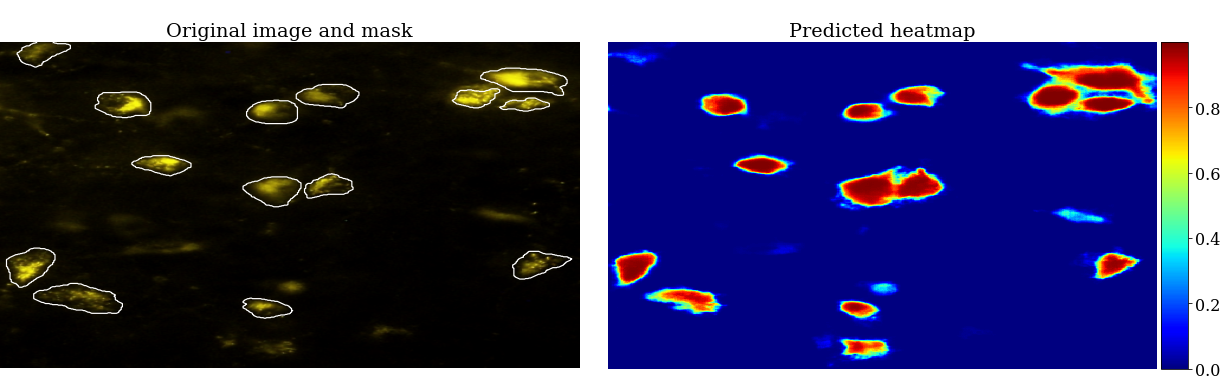
\includegraphics[width=\textwidth]{figures/130_methods/orig+heatmap:278.png}
%         \caption{
%         % Original image and raw output
%         }
%         \label{fig:raw_output}
%         \end{subfigure}
%     \begin{subfigure}{\textwidth}
%         \centering
%         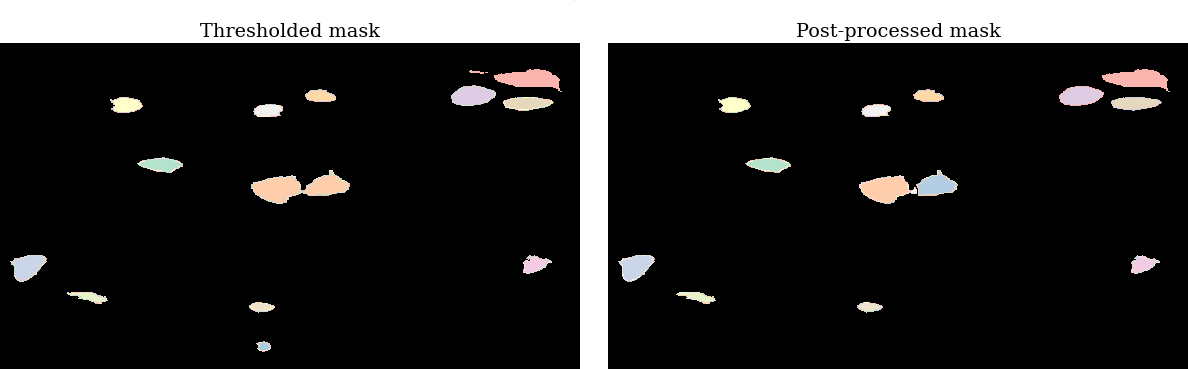
\includegraphics[width=\textwidth]{figures/130_methods/thresh+post_proc:278.png}
%         \caption{
%         % Thresholded and post-processed predicted masks
%         }
%         \label{fig:thresh+post_proc}
%         \end{subfigure}
%     \caption{\textbf{Model output}. 
%     Top: the input image with white contours indicating annotated cells  (left) and the model's raw output  (right).
%     Bottom: the predicted mask after thresholding at 0.875 (left) and the predicted mask after post-processing (right).}
%     \label{fig:model_output}
% \end{figure}
\begin{figure}
    \centering
    \subfloat[ground-truth]{
    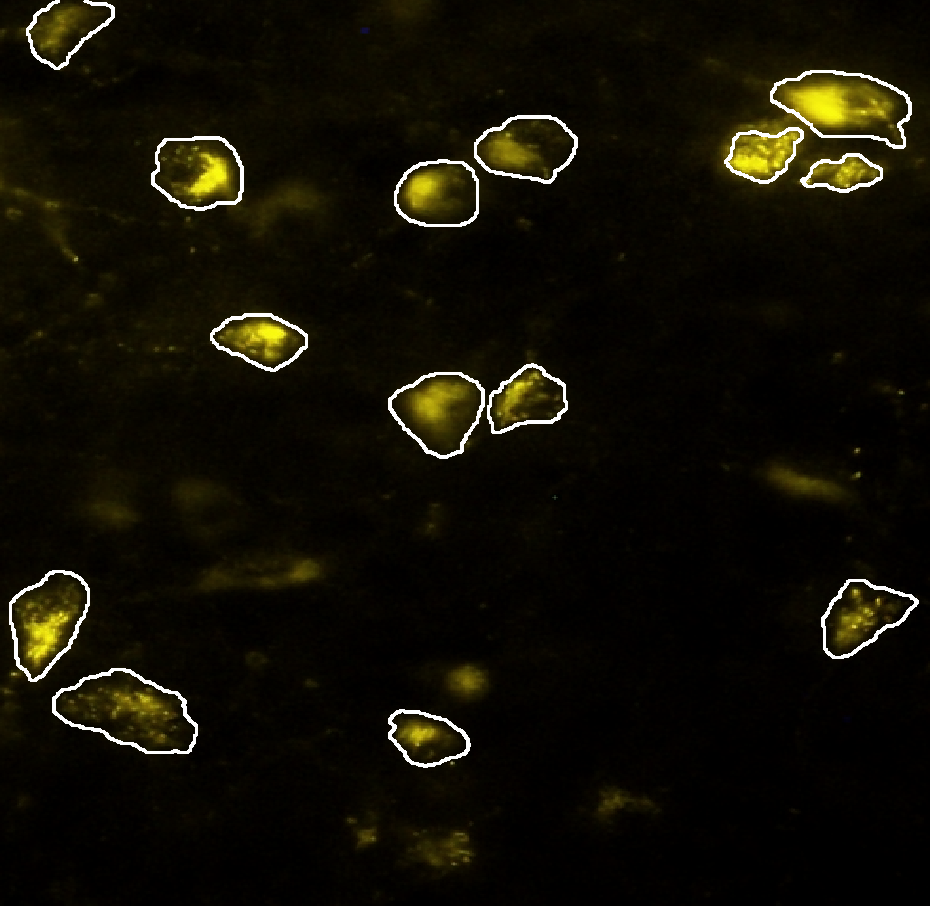
\includegraphics[width=0.5\textwidth]{figures/140_results/orig:278.pdf}\label{fig:ground_truth}
    }
    \subfloat[raw heatmap]{
    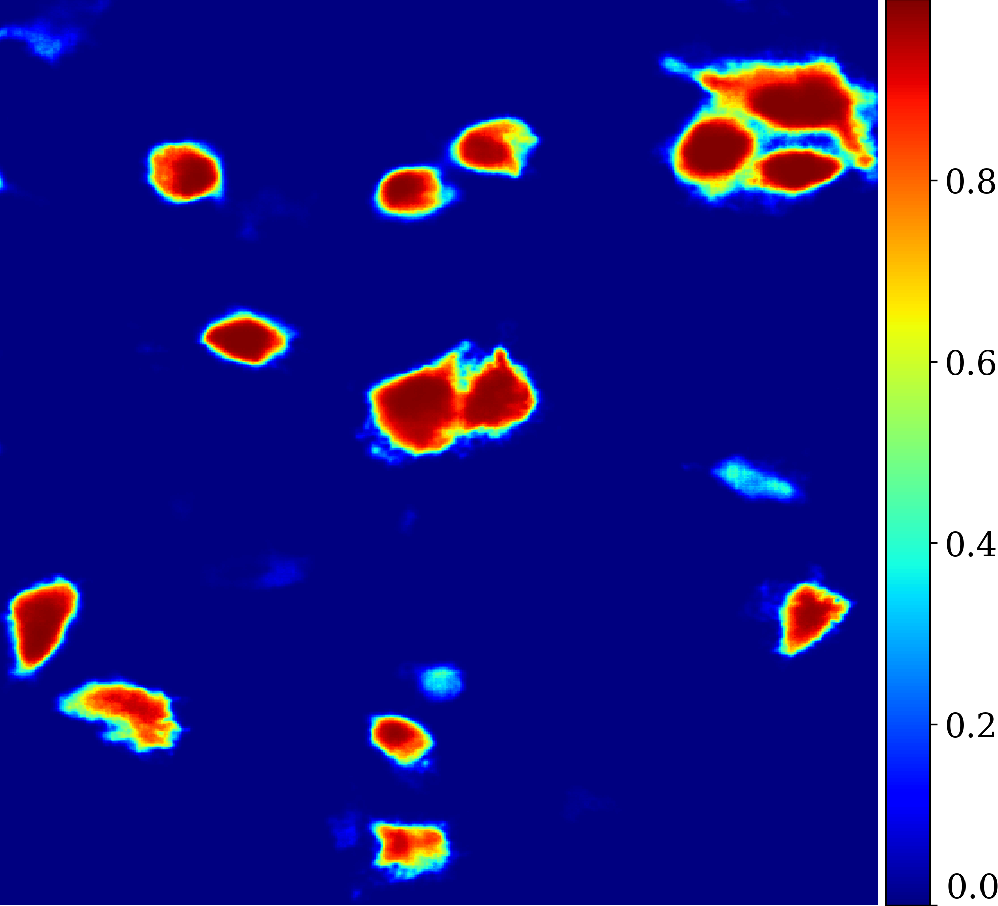
\includegraphics[%trim=0 0.008in 0 0,
    width=0.54\textwidth]{figures/140_results/heatmap:278.pdf}\label{fig:heatmap}
    }
    
    \subfloat[thresholded prediction]{
    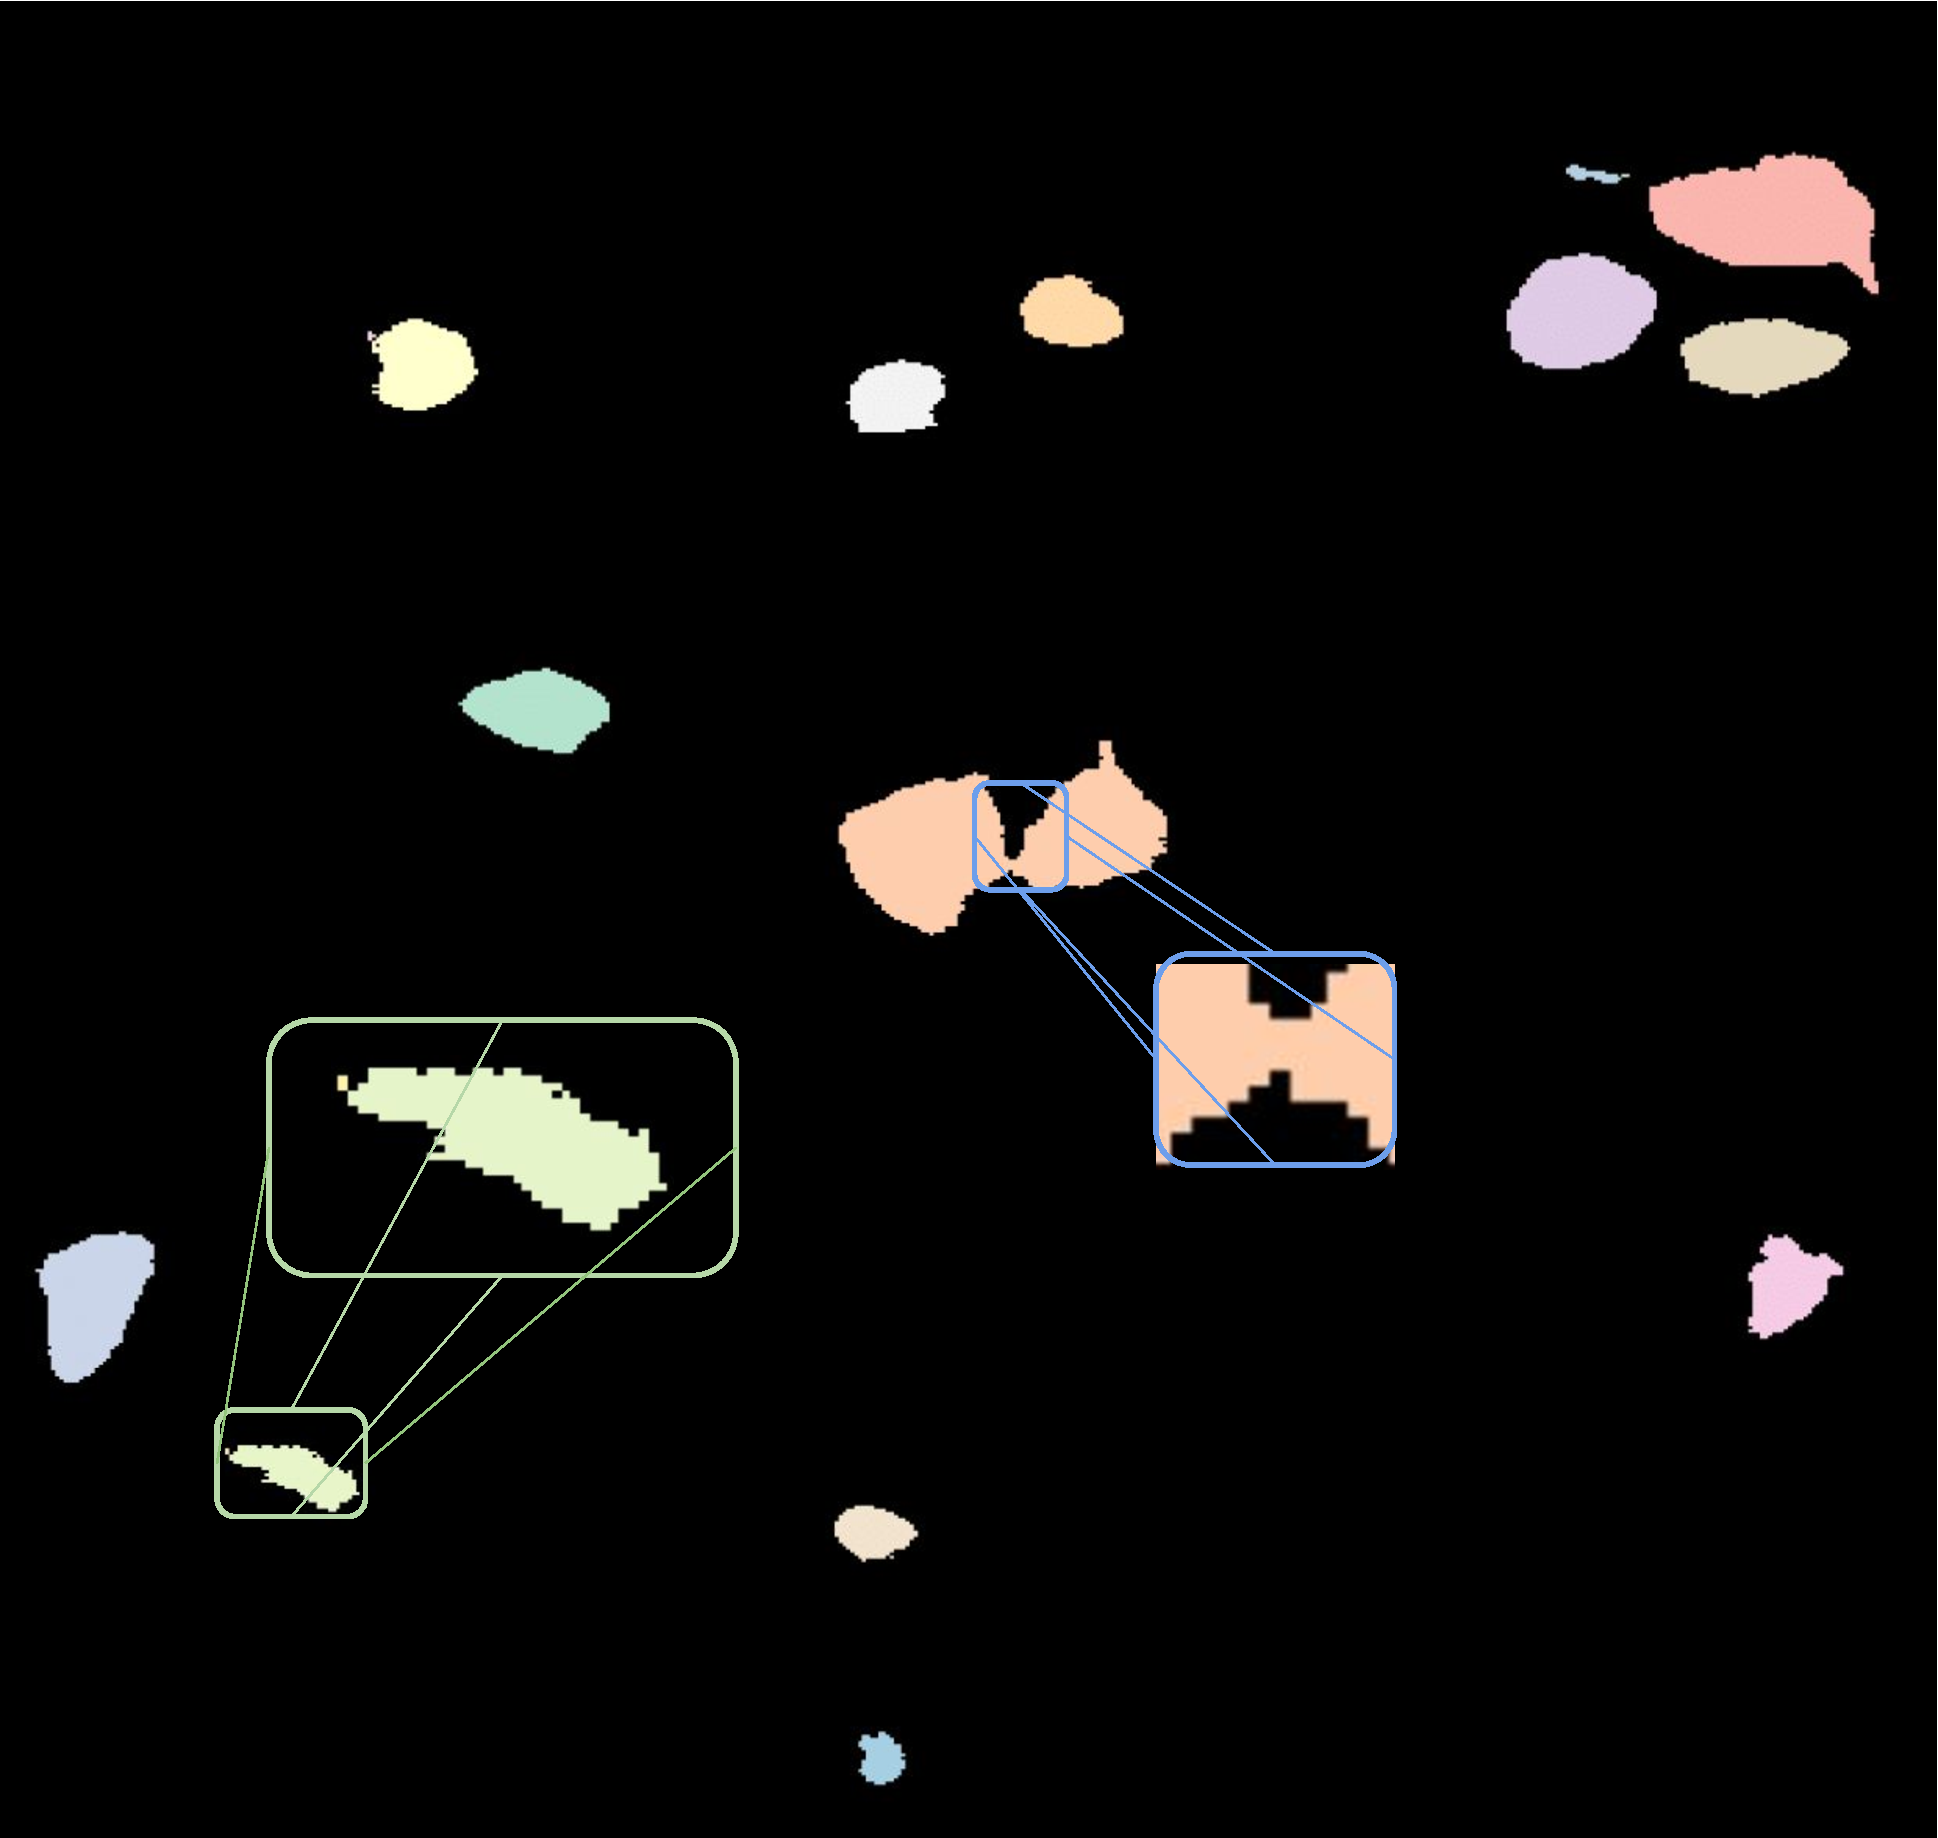
\includegraphics[width=0.5\textwidth]{figures/140_results/thresh:278_annotated.pdf}\label{fig:thresh}
    }
    \subfloat[post-processed prediction]{
    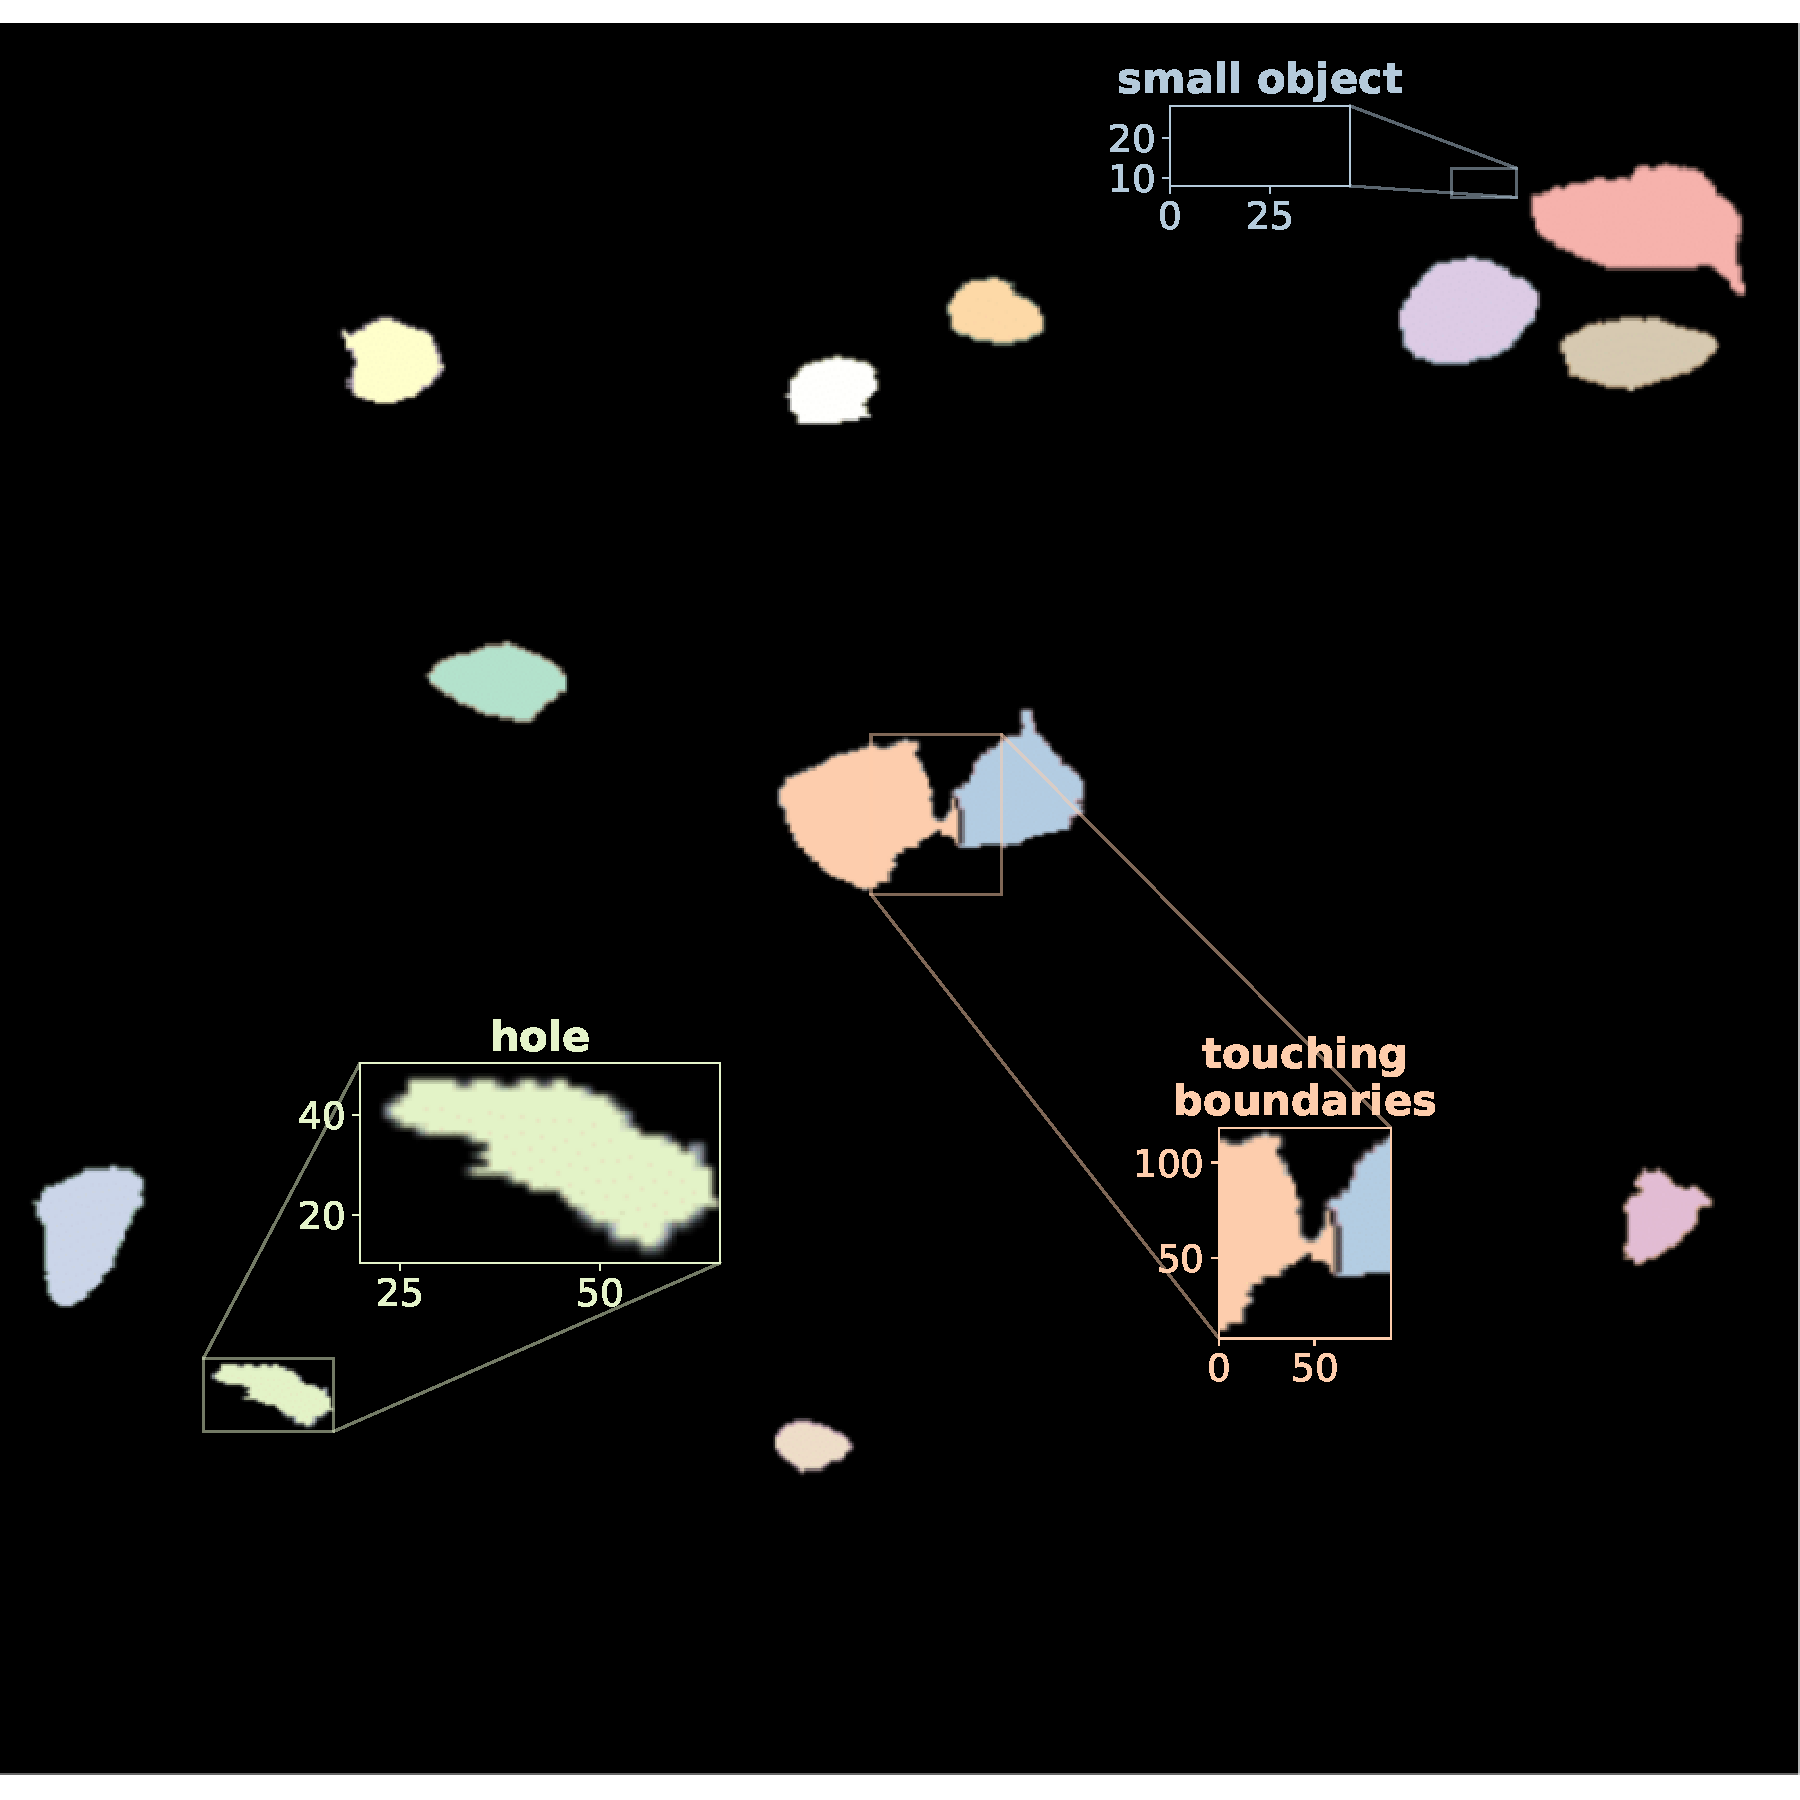
\includegraphics[width=0.5\textwidth]{figures/140_results/post_proc:278_annotated.pdf}\label{fig:post_proc}
    }
    % \subfloat[thresholded prediction]{
    % 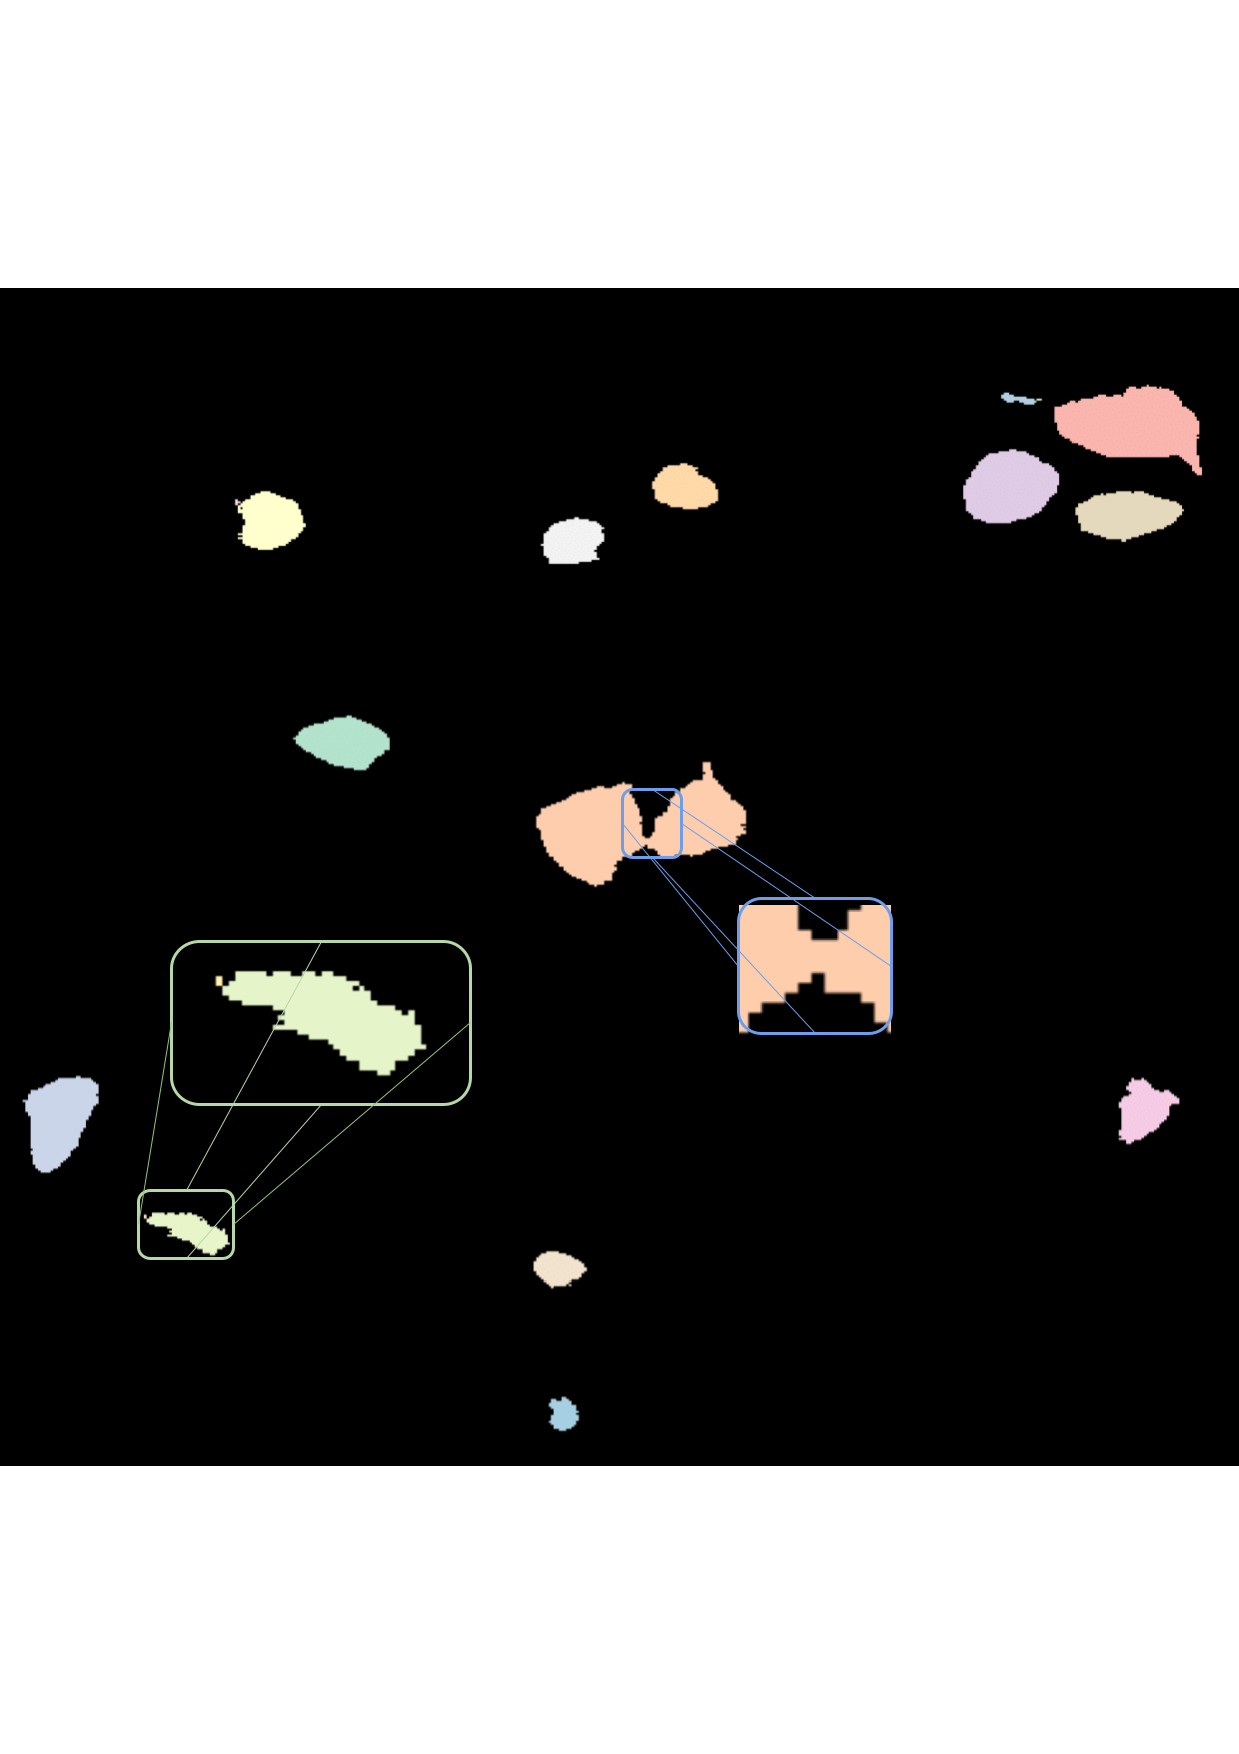
\includegraphics[width=0.5\textwidth]{figures/140_results/thresholded.pdf}\label{fig:thresh}
    % }
    % \subfloat[post-processed prediction]{
    % 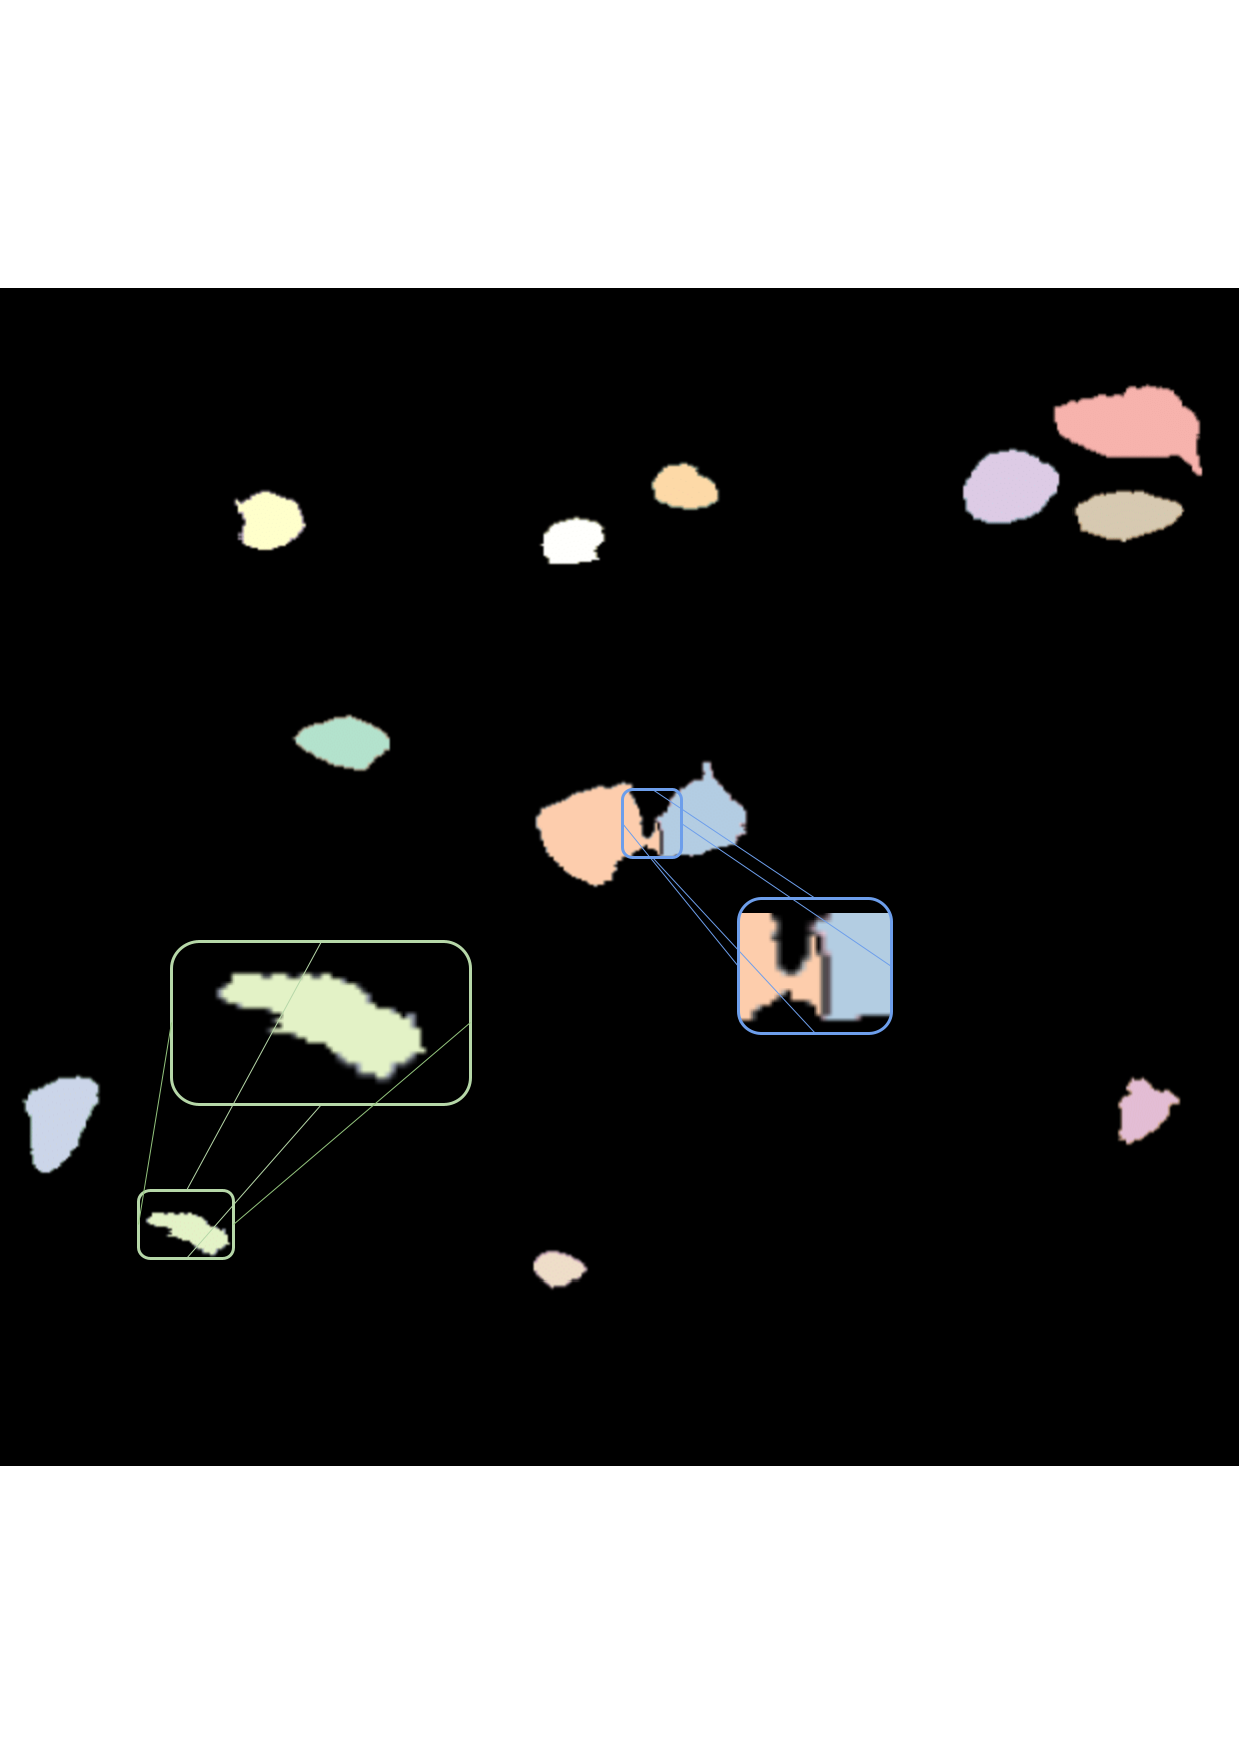
\includegraphics[width=0.5\textwidth]{figures/140_results/post-processed.pdf}\label{fig:post_proc}
    % }    
    \caption{\textbf{Model output.} 
    (\hyperref[fig:ground_truth]{a}) the input image with white contours indicating annotated cells; (\hyperref[fig:heatmap]{b}) the model's raw output; 
    (\hyperref[fig:thresh]{c}) the predicted mask after thresholding at 0.875; (\hyperref[fig:post_proc]{d}) the predicted mask after post-processing.}
    \label{fig:model_output}
\end{figure}
This section discusses the full inference pipeline adopted in our approach, with a particular focus on the post-processing impact.
\Cref{fig:model_output} reports an illustration of the above process for a sample input image (\cref{fig:ground_truth}).

% The model predicts an output mask of the same size that is possibly as close as possible to the ground-truth label produced during the annotation process (depicted as white contours in \cref{fig:ground_truth}). 
When the picture is passed through the network, the raw output consists of a probability map (or \textit{heatmap}, see \cref{fig:heatmap}) of the same size as the original input, whereby each pixel value can be interpreted as the probability of belonging to a cell. 
% An example of this outcome is reported on the right of the \ref{fig:raw_output} if the input image on the left is provided to the model.
% An example of this outcome is reported in the Fig. \ref{fig:raw_output} (right) if a sample input image (left) is provided to the model.
The higher the value, the higher is the model's confidence in classifying that pixel as the signal. 
A thresholding operation is then applied on the heatmap to obtain a binary mask where the pixels above the cutoff are represented in white (signal) and the rest in black (background).
Hence, groups of white connected pixels represent the detected cells. 
The result of thresholding for the sample image is reported in \cref{fig:thresh}, where different colors are added for visualization purposes to highlight different detected objects after the binarization.
In this case, the model seems to perform reasonably well in detecting cell instances, although not being likewise accurate in the segmentation task (cf. the white contours in \cref{fig:ground_truth} that highlight the annotated cells).
Nonetheless, some pathological behaviors are clearly visible.
First, the confidence of the model is not always uniform over all the pixels belonging to the same object.
For instance, its value is typically higher for the central regions of the detected cells and it deteriorates moving towards the boundaries, as expected.
However, this damping behavior is not always homogeneous, and a confidence decrease followed by a successive increase can be observed going towards the cell edges.
When that happens, depressed regions are formed inside the objects, and the thresholding operation risks filtering them out if their values are below the adopted cutoff.
As a result, single cells may be split into multiple instances, or their body may present internal holes.
Examples of those behaviors are the purple-ish cell in the top-right corner, for which the left tail filament has been disconnected (cf. \cref{fig:heatmap,fig:thresh}), and the green-ish object at the bottom-left, respectively. %(this is visible by zooming on the area), respectively.
Another limitation is related to the overcrowding problem discussed in \cref{sec:challenges,sec:weights_map}, as highlighted by the two close-by cells in the center of the image.
In this case, the heatmap suggests that the model cannot draw sharp boundaries around the cells, thus failing to separate them in the binary output. 

The previous observations suggest that a smarter post-processing may be required for better performances.
For this reason, we adopt ad-hoc post-processing to tackle the issues above.
In particular, we first remove isolated components of a few pixels and fill the holes inside the detected cells. 
Then, we employ the watershed algorithm \cite{watershed} to separate close-by objects.
An example of the results is provided in \cref{fig:post_proc}, where the overlapping cells in the middle of \cref{fig:thresh_opt} are correctly split after post-processing. Also, the small component in the top-right corner is removed, and the hole in the bottom-left object is filled.

Unfortunately, this step is customized for our dataset, which hinders its extension to other applications.
However, the parameters for the above operations are set quite trivially based on the average cell size.
Therefore, our approach may reasonably apply to other use cases as far as ground-truth masks are available for extracting object statistics\footnote{for more details, \postproc}.